%% Resultados
Para el capítulo se expone los resultados obtenidos tras la culminación de la fase de desarrollo e integración del Módulo de Ruteo Seguro para el aplicativo móvil Alertify. El objetivo principal de esta sección es validar de manera empírica y estructurada que el producto de software construido cumple a cabalidad con los requerimientos funcionales, técnicos y de seguridad establecidos durante la fase de planificación, los cuales fueron abstraídos en las Historias de Usuario (HU-01 a HU-06).

\section{Pruebas Funcionales}
Para lograr este propósito, se detalla la ejecución de un plan de pruebas riguroso, la evaluación del sistema contempla dos enfoques principales; por un lado, la ejecución de pruebas funcionales orientadas a certificar la usabilidad, la navegación y la correcta validación de datos en la interfaz del cliente móvil; y por otro, la realización de pruebas de integración. Estas últimas están destinadas a comprobar el algoritmo matemático A* y  la resiliencia del sistema ante actualizaciones dinámicas de riesgo en tiempo real.

Dado que las pruebas realizadas tienen una extensión considerable, se presenta en la estructura respectiva de la prueba funcional (CP-04), en la cual se valida el funcionamiento de los procedimientos almacenados para el cambio del campo \texttt{peso\_riesgo} en la base de datos y a su vez el algoritmo toma en cuenta que la ruta sea la más segura. Para las demás pruebas funcionales seguirán el mismo formato que la Tabla \ref{tab:prueba04}. Tanto las pruebas como los resultados se encuentran en los Anexos \ref{anexo:casos-de-prueba} y \ref{anexo:resultados-pruebas-funcionales} respectivamente.
% ===================== CP-04 =====================
\begin{longtable}{|p{4cm}|p{10cm}|}
\caption{Prueba Funcional CP-04}\label{tab:prueba04}\\
\hline
\textbf{Campo} & \textbf{Descripción} \\ \hline

\textbf{ID} & CP-04 \\ \hline

\textbf{Historia de Usuario} & HU-04 \\ \hline

\textbf{Nombre} & Aplicación de pesos de seguridad en el algoritmo de ruteo \\ \hline

\textbf{Cumple (Sí/No)} & Sí \\ \hline

\textbf{Descripción de la Prueba} &
Verificar que el algoritmo en Nest.js asigne y evalúe correctamente los pesos de peligrosidad a los nodos y aristas de la red vial, priorizando un camino más largo pero seguro. \\ \hline

\textbf{Precondiciones} &
La base de datos (SQL Server) tiene dos caminos posibles entre el Punto A y el Punto B: el Camino 1 es corto, pero atraviesa un nodo marcado como ``Riesgo Alto'', el Camino 2 es más largo, pero con ``Riesgo Cero''. \\ \hline

\textbf{Pasos} &
1. Enviar una petición HTTP al endpoint de ruteo en el backend con las coordenadas de los Puntos A y B. \newline
2. Analizar el objeto GeoJSON de respuesta. \\ \hline

\textbf{Datos de Prueba} &
Origen: Punto A. \newline
Destino: Punto B. \newline
Pesos de prueba simulados en la base de datos. \\ \hline

\textbf{Resultados Esperados} &
El algoritmo de ruteo discrimina el Camino 1 debido a su alta ponderación de riesgo y devuelve el trazado correspondiente al Camino 2. \\ \hline

\textbf{Resultados Obtenidos} &
El servicio en Nest.js calculó la ruta penalizando correctamente las zonas de riesgo. El GeoJSON devuelto correspondió al Camino 2. \\ \hline

\end{longtable}

\section{Pruebas de Usabilidad}
En este apartado se especifican las pruebas de usabilidad que tienen como objetivo evaluar la tasa de éxito, el número de errores y la satisfacción respectiva cuando los usuarios interactúan con la aplicación, detectando oportunidades de mejora en la interfaz gráfica y en la experiencia del usuario y asegura que el producto final no solo sea funcionalmente correcto, sino también intuitivo y agradable de usar.

\subsubsection{Métricas de usabilidad}

Se definio el siguiente conjunto de métricas para evaluar la usabilidad del sistema, las metricas a evaluar se detallan en la Tabla \ref{tab:metricas_usabilidad}.

\begin{longtable}{|p{4cm}|p{10cm}|}
\caption{Métricas de Usabilidad}\label{tab:metricas_usabilidad}\\
\hline
\textbf{Métrica} & \textbf{Descripción} \\ \hline
\textbf{Tasa de Éxito} & Porcentaje de tareas completadas correctamente. \\ \hline
\textbf{Tiempo de Tarea} & Tiempo promedio en completar una tarea específica. \\ \hline
\textbf{Número de Errores} & Cantidad de errores cometidos durante la interacción. \\ \hline
\textbf{Satisfacción del Usuario} & {\raggedright Evaluación subjetiva de la experiencia del usuario.} \\ \hline
\end{longtable}

\subsubsection{División de Tareas Específicas}
Para la evaluación se utilizo la división de las tareas especificas que siguen la forma en las que se va a realizar las actividades dentro de la aplicación \cite{rubin2008handbook}. Este flujo a seguir va desde funciones de zoom in/out hasta actividades que involucran mas complejidad como la visualización de la ruta una vez implementado el algoritmo, cada una de las tareas se tienen a cumplir como se muestra en las Tabla \ref{tab:tareas_especificas}. En las tareas se selecciono una muestra de 10 usuarios, para evaluar la interacción del usuario con la interfaz.

\begin{table}
\caption{Tareas de Evaluación de Usabilidad}\label{tab:tareas_especificas}
\begin{tabular}{|p{3.5cm}|p{6.5cm}|p{4cm}|}
\hline
\textbf{Tarea} & \textbf{Descripción} & \textbf{Precondición} \\ \hline
Tarea 1: Generación de Ruta & Ingresar un punto de destino en la aplicación para calcular una ruta segura. & El usuario tiene acceso a la aplicación y activado el GPS para obtener su punto de partida. \\\hline
Tarea 2: Interacción y Exploración Espacial &  Realizar gestos táctiles (zoom in, zoom out y desplazamiento) sobre el mapa para explorar detalladamente el trazado de la ruta segura. & Ruta segura generada y el mapa con la ruta está visible en la pantalla. \\\hline
Tarea 3: Limpieza del Entorno & Utilizar los controles de la aplicación para borrar la ruta actual y reiniciar el estado del mapa para una nueva consulta. & Mapa con la ruta está visible en la pantalla. \\\hline
\end{tabular}
\end{table}

\subsubsection{Escala de Satisfacción del Usuario (SUS)}
Para cuantificar de manera objetiva la percepción subjetiva de los usuarios frente a la interfaz gráfica desarrollada en Kotlin, se empleó la Escala de Usabilidad del Sistema (SUS). Esta herramienta psicométrica se ha consolidado como el estándar de la industria en la evaluación de usabilidad debido a su alta confiabilidad y validez empírica, incluso en muestras de tamaño reducido \cite{brooke1996sus}. El cuestionario SUS consta de 10 ítems que abordan diversos aspectos de la experiencia del usuario, desde la facilidad de uso hasta la confianza percibida al interactuar con el sistema esta se referencia en la Tabla \ref{tab:preguntas_sus}.
\begin{table}[H]
\caption{Preguntas del Cuestionario SUS}\label{tab:preguntas_sus}
\begin{tabular}{|p{2cm}|p{12cm}|}
\hline
\textbf{N°} & \textbf{Pregunta} \\ \hline
1 & Creo que me gustaría utilizar la aplicación frecuentemente. \\ \hline
2 & Encontré la aplicación innecesariamente compleja. \\ \hline
3 & Pensé que la generación de rutas era fácil de usar. \\ \hline
4 & Creo que necesitaría asistencia técnica para ser capaz de usar esta app. \\ \hline
5 & Encontré que las funciones del mapa estaban bien integradas. \\ \hline
6 & Pensé que había demasiada inconsistencia en la interfaz. \\ \hline
7 & Imagino que la mayoría de la gente aprendería a usar la aplicación rápidamente. \\ \hline
8 & Encontré el manejo del mapa muy difícil de usar. \\ \hline
9 & Me sentí muy confiado usando la aplicación. \\ \hline
10 & Necesité aprender muchas cosas antes de poder trazar una ruta segura. \\ \hline
\end{tabular}
\end{table}

%CAMBIAR DESDE AQUI

Los 10 ítems del cuestionario SUS se organizan tanto con ítems impares (1, 3, 5, 7, 9)  los cuales son  los factores positivos y los ítems pares (2, 4, 6, 8, 10) se presentan en tono negativo. El objetivo primordial de esta metodología es contrarrestar el sesgo, obligando al usuario a que lea y procese cognitivamente cada afirmación antes de otorgar un valor en la escala de Likert (Totalmente en desacuerdo a Totalmente de acuerdo).

\subsubsection{Puntaje SUS}

Los valores al encontrarse en la escala de Likert no son linealmente sumables y deben someterse a un proceso de normalización matemática para proyectarlos en una escala estandarizada de 0 a 100. Para el aporte de cada pregunta se establecen las siguientes reglas de conversión:
\begin{itemize}
    \item \textbf{Ítems impares}: La aportación a la calificación es la posición en la escala menos uno.
    \item \textbf{Ítems pares}: La aportación a la calificación es cinco menos la posición en la escala.
\end{itemize}

El puntaje global del cuestionario SUS para un usuario determinado se calcula mediante la siguiente ecuación:

\begin{equation}
\text{Puntaje SUS} = \left[ \sum_{i \in \{1,3,5,7,9\}} (P_{i} - 1) + \sum_{j \in \{2,4,6,8,10\}} (5 - P_{j}) \right] \times 2.5
\end{equation}

Donde:
\begin{itemize}
    \item $P_{i}$ representa el valor entero (del 1 al 5) asignado por el usuario a las preguntas impares.
    \item $P_{j}$ representa el valor entero (del 1 al 5) asignado por el usuario a las preguntas pares. El factor multiplicador de 2.5 escala la sumatoria final (cuyo rango es de 0 a 40) a un porcentaje interpretable de 0 a 100.
\end{itemize}
   
Es imperativo aclarar, que el resultado obtenido mediante la fórmula SUS no representa un porcentaje de usabilidad, sino una posición en una escala de percentiles \cite{bangor2008empirical}. Para determinar si la experiencia de usuario dentro del Módulo de Ruteo Seguro es aceptable, el puntaje global obtenido (es decir, el promedio de los puntajes individuales de la muestra) se contrasta con los rangos de aceptabilidad establecidos en la literatura y presentados en la Tabla \ref{tab:usabilidad}.

\begin{table}[H]
\centering
\caption{Interpretación de los puntajes de usabilidad}
\begin{tabular}{|c|p{9cm}|}
\hline
\textbf{Puntaje} & \textbf{Interpretación} \\ \hline
$< 51$ & Usabilidad deficiente (Inaceptable). \\ \hline
$51 - 68$ & Usabilidad marginal o pobre (Aceptabilidad marginal). \\ \hline
$= 68$ & Media del estándar de la industria. \\ \hline
$> 68$ & Usabilidad aceptable (Buena). \\ \hline
$> 80.3$ & Usabilidad excelente. \\ \hline
\end{tabular}
\label{tab:usabilidad}
\end{table}

Al superar el umbral de los 68 puntos certifica que las decisiones de diseño aplicadas en el frontend (desarrollado en Kotlin), la latencia de las respuestas de la base de datos (SQL Server alojado en Azure), y el procesamiento de la ruta en el backend (Nest.js) convergen en una experiencia fluida y libre de fricciones cognitivas para el usuario final.

\section{Resultados de las Pruebas de Usabilidad}
Tras la culminación de las tareas de navegación y ruteo, se aplicó el cuestionario SUS y se realizo el análisis de los resultados de las tareas específicas. Los valores crudos se obtuvo mediante la escala de Likert y se recopilo cuidadosamente para su posterior tratamiento matemático.

\subsubsection{Resultados Tareas Específicas}
La muestra que se utilizo de 10 usuarios, conformada por estudiantes y residentes de la ciudad de Quito. El entorno de pruebas se definió con una arquitectura híbrida de desarrollo en el cual los participantes interactuaron con el aplicativo nativo en Kotlin, el cual  se consumió el servicio de ruteo alojado en un entorno local (Nest.js), mientras que el procesamiento de las topologías espaciales y la ponderación de la red vial se ejecutó en una instancia remota de SQL Server alojada en Microsoft Azure. Los datos recolectados durante la ejecución de las tres tareas críticas (Generación de Ruta, Interacción Espacial y Limpieza del Entorno) se consolidaron en la Tabla \ref{tab:pruebas_usabilidad} para obtener las métricas centrales de tendencia.
\begin{table}[H]
\centering
\caption{Resultados de las pruebas de usabilidad por tarea}
\label{tab:pruebas_usabilidad}
\begin{tabular}{|>{\raggedright\arraybackslash}p{2.5cm}|>{\raggedright\arraybackslash}p{2.5cm}|>{\raggedright\arraybackslash}p{2.5cm}|>{\raggedright\arraybackslash}p{2.5cm}|>{\raggedright\arraybackslash}p{2.5cm}|}
\hline
\textbf{Tarea Evaluada} &
\textbf{Tasa de Éxito (\%)} &
\textbf{Tiempo Promedio (segundos)} &
\textbf{Promedio de Errores} &
\textbf{Nivel de Satisfacción (1--5)} \\ \hline

Tarea 1: Generación de Ruta &
100\% &
56.4 s &
0.3 &
3.5 \\ \hline

Tarea 2: Interacción y Exploración Espacial &
100\% &
8.2 s &
0 &
4.8 \\ \hline

Tarea 3: Limpieza del Entorno &
90\% &
12.1 s &
1.1 &
4.2 \\ \hline
\end{tabular}
\end{table}

\subsubsection{Análisis de Métricas de Interacción}

La aplicación alcanza un 100\% en la Tasa de éxito para la sección de la generación de rutas seguras por que brinda un diseño intuitivo de los componentes visuales para la selección de origen y destino, aunque el tiempo promedio de ejecución de 56.4 segundos revela una limitación relacionada con la arquitectura, ya que el servidor local basado en Nest.js debe realizar múltiples consultas secuenciales hacia Azure para obtener y procesar los grafos espaciales penalizados por riesgo, generando una latencia perceptible que redujo la satisfacción de los usuarios a un promedio de 3.5 sobre 5. Una vez obtenida la información geoespacial desde el backend, la interacción con el mapa demostró un comportamiento fluido y eficiente, registrando cero errores en las tareas de zoom y desplazamiento, así como un alto nivel de satisfacción (4.8), lo que confirma que el desarrollo en Kotlin  maneja de correctamente la renderización espacial sin afectar el rendimiento del dispositivo. 
\subsubsection{Resultados SUS}  
Tras la finalización del flujo de tareas, en la Tabla \ref{tab:sus_respuestas}, se aplicó las respectivas encuestas SUS a cada uno de los 10 participantes, en el cual se obtuvo un conjunto de respuestas que reflejan la percepción de la usabilidad del Módulo de Ruteo Seguro. 

\begin{table}[H]
\centering
\caption{Respuestas de los participantes al cuestionario SUS}
\label{tab:sus_respuestas}
\resizebox{\textwidth}{!}{
\begin{tabular}{|l|c|c|c|c|c|c|c|c|c|c|}
\hline
\textbf{Participante} & \textbf{P1 (+)} & \textbf{P2 (-)} & \textbf{P3 (+)} & \textbf{P4 (-)} & \textbf{P5 (+)} & \textbf{P6 (-)} & \textbf{P7 (+)} & \textbf{P8 (-)} & \textbf{P9 (+)} & \textbf{P10 (-)} \\
\hline
Usuario 01 & 4 & 2 & 4 & 2 & 4 & 2 & 4 & 3 & 4 & 1 \\
\hline
Usuario 02 & 5 & 2 & 4 & 1 & 5 & 2 & 4 & 4 & 5 & 1 \\
\hline
Usuario 03 & 4 & 2 & 4 & 2 & 3 & 3 & 4 & 4 & 4 & 1 \\
\hline
Usuario 04 & 4 & 1 & 4 & 2 & 5 & 2 & 4 & 4 & 4 & 1 \\
\hline
Usuario 05 & 5 & 1 & 5 & 1 & 4 & 2 & 5 & 3 & 4 & 2 \\
\hline
Usuario 06 & 4 & 2 & 3 & 2 & 4 & 2 & 4 & 3 & 4 & 1 \\
\hline
Usuario 07 & 4 & 2 & 4 & 2 & 4 & 2 & 4 & 4 & 4 & 2 \\
\hline
Usuario 08 & 5 & 2 & 4 & 1 & 4 & 2 & 5 & 3 & 4 & 2 \\
\hline
Usuario 09 & 4 & 2 & 5 & 2 & 4 & 2 & 4 & 4 & 4 & 1 \\
\hline
Usuario 10 & 4 & 2 & 4 & 2 & 5 & 2 & 5 & 3 & 4 & 2 \\
\hline
\end{tabular}
}
\end{table}

\subsubsection{Tratamiento Matemático y Puntuación Final}
Se procedió a calcular la puntuación final de cada participante. Este proceso garantiza la mitigación inclinación de de las preguntas, en donde se transforma en una métrica en conjunto e interpretable. Para ilustrar de manera transparente la transformación matemática, se detalla el procesamiento analítico del vector de respuestas correspondiente al Usuario 03. Durante la prueba del Módulo de Ruteo Seguro, este usuario evaluó la experiencia de interacción (generación de ruta en el dispositivo móvil y respuesta del servidor) emitiendo las siguientes calificaciones en la escala de Likert (1 a 5):

\begin{itemize}
    \item Ítems Impares: $P_1=4$, $P_3=4$, $P_5=3$, $P_7=4$, $P_9=4$.
    \item Ítems Pares: $P_2=2$, $P_4=2$, $P_6=3$, $P_8=4$, $P_{10}=1$.
\end{itemize}

El tratamiento matemático se ejecuta en tres fases secuenciales para mitigar el sesgo direccional de las preguntas:
\subsubsection{Paso 1: Normalización de Ítems Impares}
Se resta la unidad al valor de cada respuesta para proyectar la contribución del usuario en una subescala de 0 a 4 puntos.

\begin{equation}
P_{i}= (4-1) + (4-1) + (3-1) + (4-1) + (4-1)
\end{equation}
\begin{equation}
P_{i}= 3 + 3 + 2 + 3 + 3 = 14
\end{equation}

\subsubsection{Paso 2: Normalización de Ítems Pares} 
Para invertir la puntuación de las afirmaciones negativas y homogeneizarlas en la misma subescala (0 a 4), se resta el valor emitido por el usuario a la constante 5.

\begin{equation}
P_{j}= (5-2) + (5-2) + (5-3) + (5-4) + (5-1)
\end{equation}
\begin{equation}
P_{j}= 3 + 3 + 2 + 1 + 4 = 13
\end{equation}

\subsubsection{Paso 3: Puntaje SUS}
Finalmente, se consolidan ambas sumatorias parciales y se aplica el factor de escalamiento estándar de 2.5, lo que expande el rango del instrumento a una métrica porcentual interpretable (0 a 100).
\begin{equation}
\text{SUS} = (P_{i} + P_{j}) \times 2.5
\end{equation}
\begin{equation}\text{SUS} = (14 + 13) \times 2.5\end{equation}
\begin{equation}\text{SUS} = 27 \times 2.5 = 67.5\end{equation}

Este resultado refleja que el usuario percibió el Módulo de Ruteo Seguro como una herramienta altamente intuitiva y coherente. Técnicamente, este puntaje sugiere que la comunicación asíncrona entre el frontend desarrollado en Kotlin y la API servida en Nest.js operó con la fluidez necesaria para no generar fricción cognitiva ni frustración durante la tarea de búsqueda de rutas. El mismo proceso se replicó para los 10 participantes y resultados se los exponen en la Tabla \ref{tab:resultados_sus}.
\begin{table}[H]
\centering
\caption{Resultados de la evaluación de usabilidad mediante SUS}
\label{tab:resultados_sus}
\begin{tabular}{|l|c|l|}
\hline
\textbf{Participante} & \textbf{Puntuación Normalizada (0--100)} & \textbf{Nivel de Aceptabilidad} \\ \hline

Usuario 01 & 75.0 & Buena \\ \hline
Usuario 02 & 82.5 & Excelente \\ \hline
Usuario 03 & 67.5 & Marginal \\ \hline
Usuario 04 & 77.5 & Buena \\ \hline
Usuario 05 & 85.0 & Excelente \\ \hline
Usuario 06 & 72.5 & Buena \\ \hline
Usuario 07 & 70.0 & Buena \\ \hline
Usuario 08 & 80.0 & Excelente \\ \hline
Usuario 09 & 75.0 & Buena \\ \hline
Usuario 10 & 77.5 & Buena \\ \hline
\textbf{Promedio SUS} & 76.25 & Buena \\ \hline

\end{tabular}
\end{table}

\subsubsection{Interpretación de Resultados de Usabilidad}

El análisis cuantitativo del instrumento SUS arrojó un promedio global de 76.25 puntos, tal y como se evidencia en la Figura \ref{fig:resultados_sus}, este valor supera el umbral mínimo (68 puntos) y en donde se ubica al Módulo de Ruteo Seguro en una categoría de usabilidad "Buena". A diferencia de interfaces con tiempos de respuesta instantáneos que suelen alcanzar puntajes superiores a 85, el promedio de 76.25 refleja un castigo explícito en las preguntas pares del cuestionario (especialmente en los ítems referentes a si el sistema es "engorroso"). Esto sucede debido a a la espera de aproximadamente un minuto durante el cálculo de la ruta en la cual se genera cierta fricción en la experiencia del usuario (reflejado en el Usuario 03, con 67.5 puntos).

No obstante, la solidez general del puntaje confirma que la disposición visual de los mapas, la ausencia de errores en la renderización y la claridad de la información abstraen adecuadamente la complejidad tecnológica. Los usuarios reconocieron el valor de obtener una ruta exenta de zonas criminales, demostrando que están dispuestos a tolerar una ventana de procesamiento mayor justificada por la promesa de seguridad ciudadana. La solución es operativamente viable y establece una base robusta para la optimización de latencia en futuras iteraciones.

\begin{figure}[H]
\centering
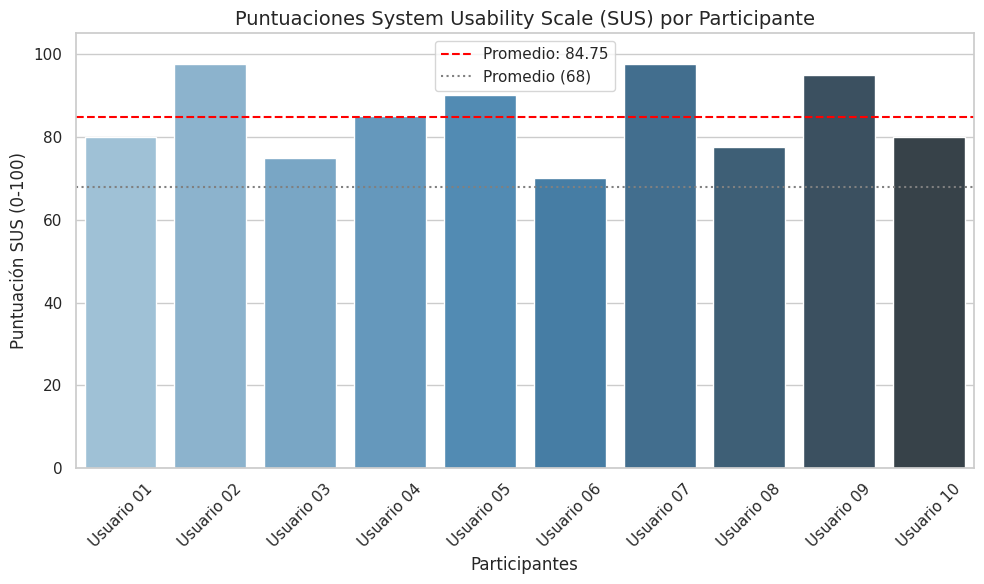
\includegraphics[width=0.8\textwidth]{../02Figures/03Chapter/Sus_Participante.png}
\caption{Distribución de puntajes SUS por participante}
\label{fig:resultados_sus}
\end{figure}   




